\chapter{Grundlagen}\label{sec:grundlagen}
\section{Python}\label{sec:python}
Anwendungen für den Roboter Pepper (Kapitel \ref{sec:pepper}) können in Python,
C++, Java, JavaScript oder ROS programmiert werden. \cite{SoftBankIII2018} Bei
den bisherigen Anwendungen wurde Python als Programmiersprache verwendet.
Deshalb wird auch für diese Anwendung als
hauptsächliche Programmiersprache verwendet. "`Python ist eine portable,
interpretative, objektorientiere Programmiersprache"' \cite{Weigend2017}. Ihre
Entwicklung wurde 1989 von Guido van Rossum begonnen. Heute wird die Entwicklung
von der nichtkommerziellen Organisation "`Python Software Foundation"'
\footnote{\url{https://www.python.org/psf/}} koordiniert.

\subparagraph{}
Das Python-Skript wird von einem Interpreter ausgeführt. Python-Skripte können
auf verschiedenen Systemplattformen (Unix, Windows, Mac OS) ausgeführt werden.
Deshalb bezeichnet man Python als portable Sprache. Zudem gilt Python-Code als
sehr gut lesbar und ein Programm kann mit weniger Code erstellt
werden als in anderen Programmiersprachen. Listing \ref{lst:python-hello-world}
zeigt ein "`Hello World"'-Programm in Python im Vergleich zu einem Java-Programm
in Listing \ref{lst:java-hello-world}, welches die gleiche Funktion umfasst.
Die aktuelle Python Version ist 3.6.
Da auf dem Roboter allerdings Python 2.7 installiert ist, wird die Anwendung mit
dieser Version entwickelt. \cite{Weigend2017}

\begin{lstlisting}[float, language=Python, frame=single, framexleftmargin=15pt,
style=algoBericht, label={lst:python-hello-world}, captionpos=b, caption={Hello
World in Python}]
print "Hello, world!"
\end{lstlisting}

\begin{lstlisting}[float, language=Java, frame=single, framexleftmargin=15pt,
style=algoBericht, label={lst:java-hello-world}, captionpos=b, caption={Hello
World in Java}]
public class HelloWorld { 
	public static void main(String[] args) {
		System.out.println("Hello, world!"); 
	}
}
\end{lstlisting}

\section{PowerPoint}\label{sec:powerpoint}
Microsoft PowerPoint ist ein Quasistandard für das Erstellen von
computergestützten Präsentationen. PowerPoint ist die bekannteste Software zum
erstellen von Präsentationsfolien. Die Benutzung von
PowerPoint wird als einfach zu erlnernen angesehen. \cite{Thielsch2012} Auch in
der Fiducia \& GAD ist PowerPoint Teil der Distribution des Bankarbeitsplatz.
Somit steht die Anwendung den Bankmitarbeitern zur Verfügung. Es ist also
naheliegend für das Erstellen von Präsentationen, die von Pepper vorgestellt
werden sollen, zu verwenden.

%% Ich würde hier etwas über die allgemeine Verbreitung von Powerpoint schreiben
%% und darauf hinweisen, dass auch wir (Fiducia GAD) im Rahmen der Distribution
%% des Bankarbeitsplatzes Powerpoint ausrollen. Es ist daher naheliegend
%% anzunehmen, dass Powerpint ein einfach zu bedienendes Frontend für den
%% Kundenkreis darstellt.
%%
%% http://www.thielsch.org/download/paper/Thielsch_Perabo_2012.pdf


\section{Flask}\label{sec:flask}
Flask ist ein Mikroframework für Python zum Erstellen von Webanwendungen. Es ist
möglichst einfach aufgebaut, aber umfasst trotzdem alle nötigen Funktionen.
Einfache Anwendungen können mit Flask schnell erstellt werden. \cite{Flask2018}
Listing \ref{lst:flask-simpel} zeigt den Aufbau einer einfachen Webanwendung, die mit
Hilfe von Flask auf der Startseite "`Hello, world!"' ausgibt.
\texttt{@app.route("'/"')} gibt an, welchen Pfad der Benutzer aufrufen muss,
damit die entsprechende Methode (in diesem Fall \texttt{hello()}) ausgeführt
wird. Mit \texttt{app.run()} wird der Server gestartet. Durch die Verwendung von
\texttt{return render\_template("'hello.html"')} können HTML-Dateien (in diesem
Beispiel die Datei "`hello.html"') dargestellt werden. So lässt sich eine
Webanwendung entwickeln, die beim Aufruf verschiedener Pfade jeweils eine
HTML-Webseite darstellt.

\begin{lstlisting}[float, language=Python, frame=single, framexleftmargin=15pt,
style=algoBericht, label={lst:flask-simpel}, captionpos=b, caption={Einfache
Webanwendung, die auf der Startseite "`Hello, world!"' ausgibt}]
from flask import Flask
app = Flask(__name__)

@app.route("/")
def hello():
	return "Hello, world!"

if __name__ == "__main__":
	app.run()
\end{lstlisting}

\section{Verteilte Systeme}
\subsection{Client}
Ein Client ist eine Ausführungseinheit, die mit einem Server in einer
Konsumenten-Produzenten-Beziehung steht. Der Client dient als Konsument. Er
stellt Anfragen zu Diensten oder Informationen an den Server. Die Antwort auf
diese Anfragen werden vom Client zu seinem eigenen Zweck und zur Erledigung
seiner Aufgabe verwendet. Clients sind auslösende Prozesse, auf die ein Server
reagieren kann. Sie können Aktivitäten zu beliebigen Zeiten initiieren.
\cite{Bengel2015}

\subsection{Server}
Der Server dient in der Konsumenten-Produzenten-Beziehung als Produzent. Er
bearbeitet die Daten- und Dienstanfragen, die durch einen Client gestellt
werden. Ein Server ist ein reagierender Prozess. Er wartet auf Anfragen durch
einen Client und reagiert darauf, sobald eine Anfrage gestellt wird. Nach dem
Bearbeiten sendet der Server das Ergebnis an den entsprechenden Client zurück.

\subparagraph{}
Die Interaktion zwischen den Clients und
dem Server verlaufen somit nach einem fest vorgegebenen Protokoll: Der Client
sendet eine Anforderung (Request) an den Server, dieser erledigt die Anforderung
oder Anfrage und schickt eine Rückantwort (Reply) zurück an den Client. Der
Server stellt somit einen zentralen Punkt dar, an den Anforderungen geschickt
werden können
\cite{Bengel2015}

\subsection{Client-Server-Modell}
Client-Server-Systeme bestehen aus einem Server und einem oder mehreren Clients.
Dabei können Clients und Server auf unterschiedlichen aber auch auf dem gleichen
Rechner laufen. Client und Server haben unterschiedliche Zuständigkeitsbereich,
diese sind ihnen jeweils fest zugeordnet. Zusammen bilden diese Einheiten ein
komplettes System. Ein Server kann mehrere Clients bedienen. Die Clients haben
keine Kenntnis voneinander. Der einzige Bezug zueinander ist, dass sie den
gleichen Server verwenden.

\subparagraph{}
Die Interaktion zwischen Client und Server laufen nach einem fest vorgegebenen
Protokoll ab. "`Der Client sendet eine Anforderung (Request) an den Server,
dieser erledigt die Anforderung oder Anfrage und schickt eine Rückantwort
(Reply) zurück an den Client."'
\cite{Bengel2015}

\section{MQTT}\label{sec:mqtt}
\ac{mqtt} ist ein lizenzfreies Protokoll zum Austausch von Nachrichten. Es ist
simpel aufgebaut und wurde für die Verwendung zwischen Geräten mit geringer
Funktionalität entwickelt. Da \ac{mqtt} ein sehr robustes Protokoll ist, eignet
es sich gut für unzuverlässige Netze mit geringer Bandbreite und hoher
Latenzzeit. \ac{mqtt} bietet eine hohe Zuverlässigkeit und minimiert die
genutzte Bandbreite. Aufgrund dieser Eigenschaften wird \ac{mqtt} z.~B.
bei Sensornetzwerken, Machine to Machine, Telemedizin, Patientenüberwachung und
dem "`Internet der Dinge"' eingesetzt.

\subparagraph{}
Das Protokoll wurde 1999 von IBM für die
Satellitenkommunikation entwickelt. Später wurde es auch in vielen weiteren
industriellen Anwendungen eingesetzt.

\subparagraph{}
\begin{figure}
  \centering
     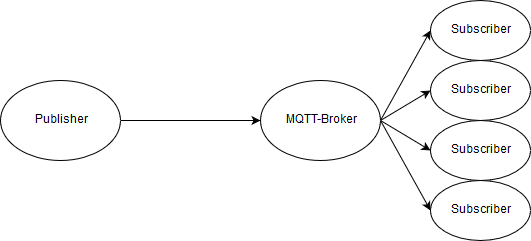
\includegraphics[width=\textwidth]{mqtt-struktur}
  \caption{Struktur von \ac{mqtt}}
  \label{fig:mqtt}
\end{figure}

Die Struktur von \ac{mqtt} (vgl. Abb. \ref{fig:mqtt}) besteht aus einem Publisher,
einem Subscriber und einem Message-Broker. Der Publisher sendet Nachrichten, der Subscriber
empfängt bestimmte Nachrichten. Der Message-Broker dient als
Kommunikationssteuerung und sorgt für das Verteilen der Nachrichten, welche von
einem Publisher gesendet werden. Der Subscriber kann ein bestimmtes Topic
(Thema) subscriben (abonnieren). Ein Publisher sendet eine Nachricht, die das
Thema und einen Inhalt beinhaltet, an den Message-Broker. Dieser sendet die
Nachricht an alle Subscriber, die das Thema der Nachricht abonniert haben.
\cite{dennisseidel2018}

%% TODO
%% Sicherlich ist es noch interessant ein bisschen auf die Programmierung von
% Pepper einzugehen. Also NAOqi und genauer, wie man Pepper sprechen lässt und
% vielleicht auch Ausgabe auf dem Tablet
\section{Programmierung von Pepper}\label{sec:programmierung-von-pepper}
Um Anwendungen für Pepper zu programmieren, wird das NAOqi Modul für Python
verwendet. NAOqi ist das Betriebssystem %TODO Stimmt das???
von Pepper. Über die \ac{api} des Roboters, kann er gesteuert werden und auf
seine Funktionen zugegriffen werden. So kann er sprechen und auf seinem Tablet
können Ausgaben angezeigt werden. Dazu werden Services aufgerufen, die eine
bestimmte Funktion von Pepper steuern. Für das Sprechen wird der Service
\texttt{ALAnimatedSpeech} verwendet. Mit \texttt{ALAnimatedSpeech.say()} wird
dem Roboter ein Text übergeben, den er vorliest. Auf dem Tablet können Webseiten
angezeigt werden. Mit dem Service \texttt{ALTabletService} wird das Tablet
gesteuert. Eine Webseite kann mit \texttt{ALTabletService.showWebview()}
angezeigt werden.
